\section{Potrzebne biblioteki}
\sectionauthor{Katarzyna Rugiełło}

Poniżej znajduje się lista bibliotek, niezbędnych do korzystania ze zbudowanej aplikacji.

\begin{enumerate}
\item numpy
\item matplotlib
\item pygame
\item os
\item scipy
\item time
\item sympy
\end{enumerate}

W przypadku, w którym którakolwiek z bibliotek nie byłaby zainstalowana można to zrobić bezpośrednio z poziomu IDE. W tym celu należy z pasku górnego wybrać zakładkę ,,File''

\begin{figure}[h]
\centering
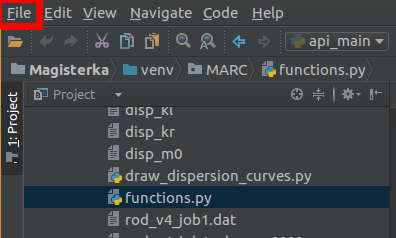
\includegraphics[width=10cm]{Zdjecia/5/kasia/file2}
\caption{Zakładka "File"}
\label{fig:file}
\end{figure}

Następnie z paska wybrać opcję ,,Settings''

\begin{figure}[h]
\centering
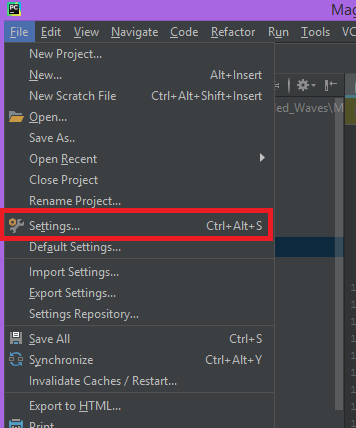
\includegraphics[width=10cm]{Zdjecia/5/kasia/settingsA}
\caption{Zakładka ,,Settings''}
\label{fig:file}
\end{figure}

W nowo otwartym oknie należy znaleźć zakładkę z nazwą bieżącego projektu.

\begin{figure}[h]
\centering
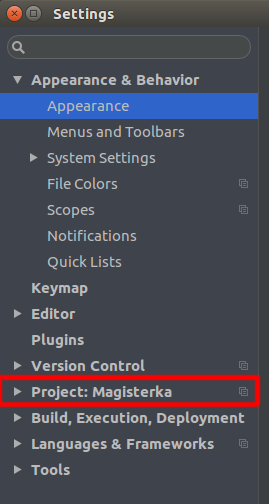
\includegraphics[width=8cm]{Zdjecia/5/kasia/settings2A}
\caption{Okno ustawień}
\label{fig:file}
\end{figure}

Z rozwijanego menu należy wybrać ,,Project interpreter''. Następnie należy nacisnąć prawym przyciskiem myszy na symbolu zielonego plusa.

\begin{figure}[h]
\centering
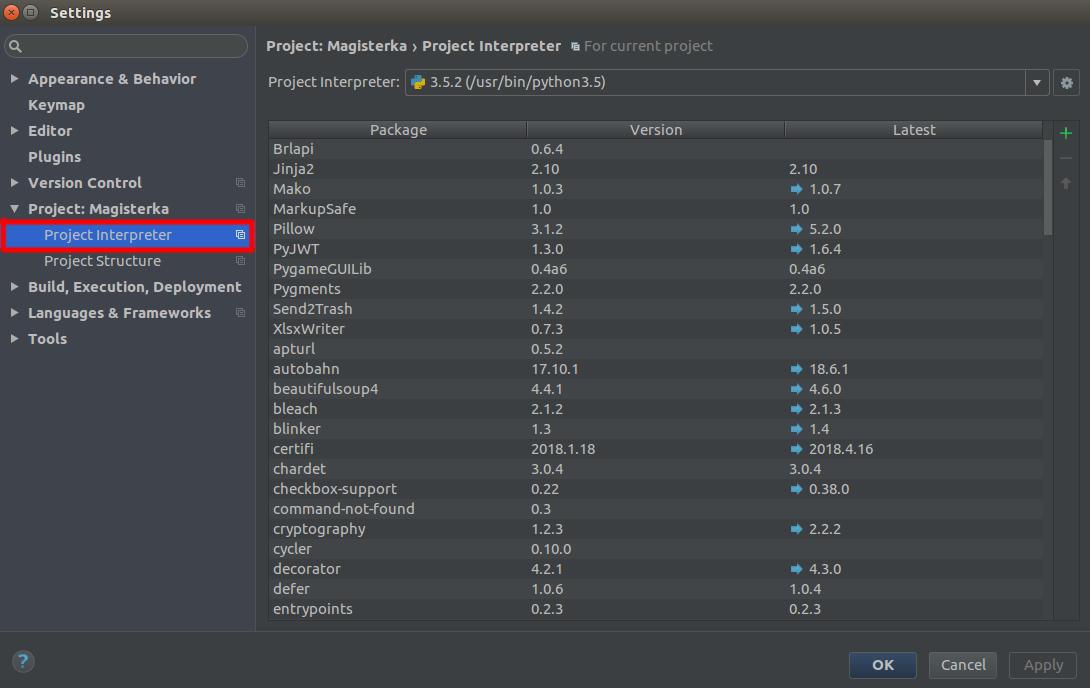
\includegraphics[width=13cm]{Zdjecia/5/kasia/settings3}
\caption{Okno interpretera}
\label{fig:file}
\end{figure}

\begin{figure}[h]
\centering
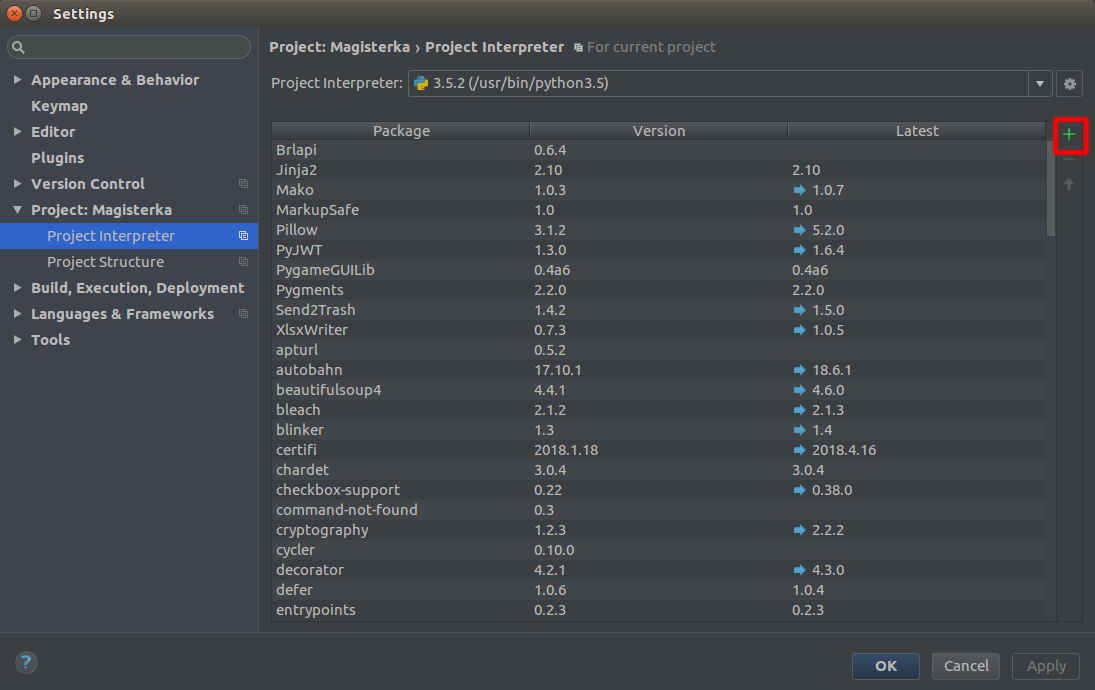
\includegraphics[width=13cm]{Zdjecia/5/kasia/settings4}
\caption{Ikona instalacji}
\label{fig:file}
\end{figure}

W nowo otwartym oknie w polu wyszukiwania, należy wpisać nazwę biblioteki, która ma zostać zainstalowana. Następnie należy nacisnąć przycisk "Install Package"

\begin{figure}[h]
\centering
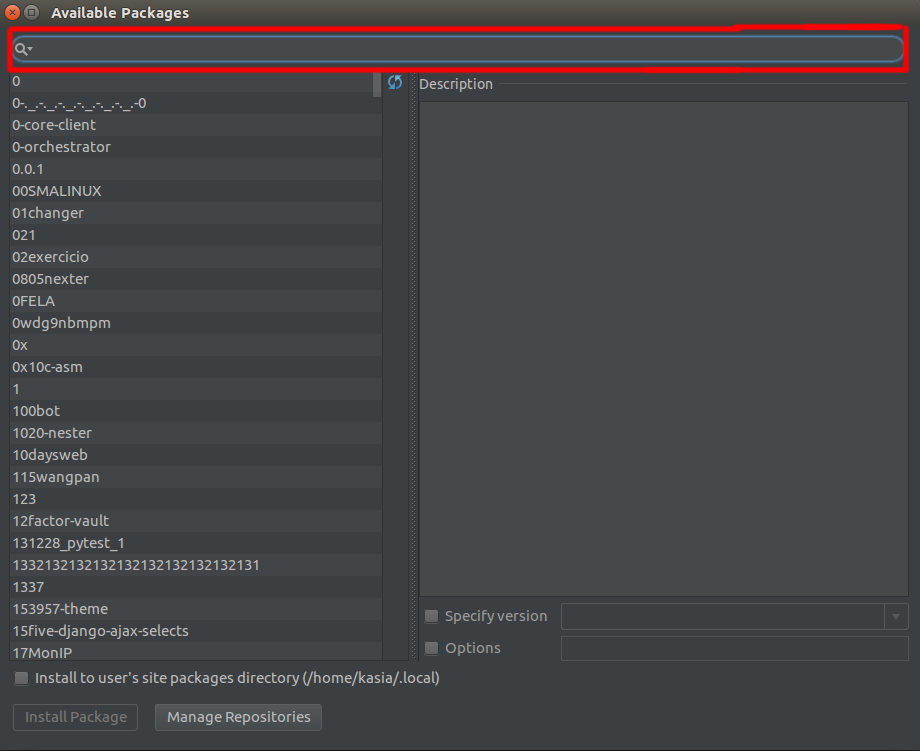
\includegraphics[width=13cm]{Zdjecia/5/kasia/settings5}
\caption{Wyszukiwanie bibliotek}
\label{fig:file}
\end{figure}

\begin{figure}[h]
\centering
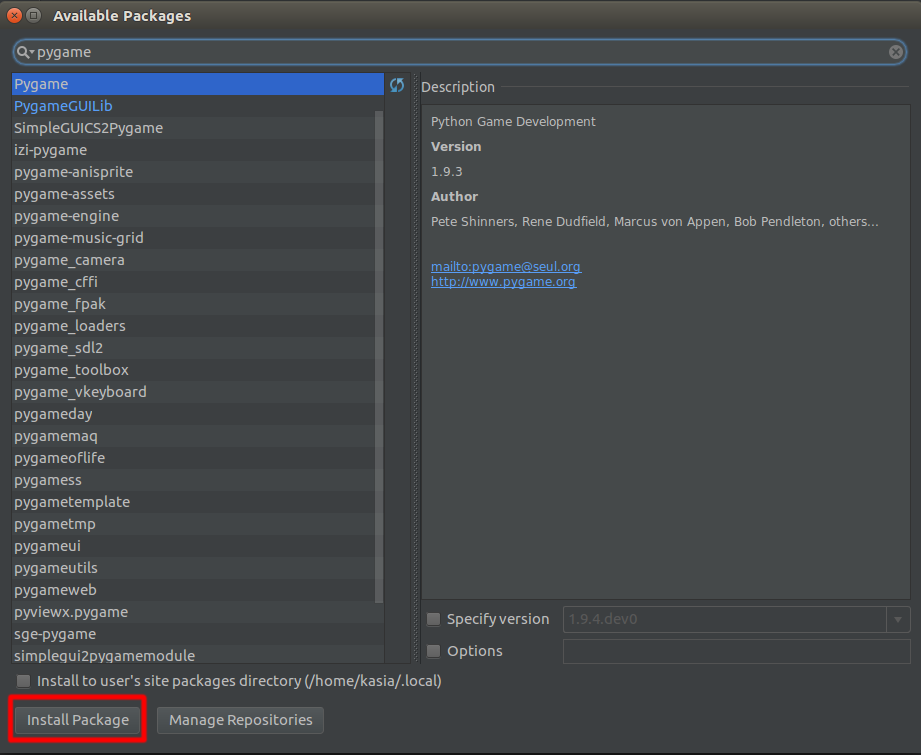
\includegraphics[width=13cm]{Zdjecia/5/kasia/settings6}
\caption{Instalacja}
\label{fig:file}
\end{figure}